\chapter{Related Work}

\section{Related Work for Parikshan}


\subsection{Record and Replay Systems:}  
Record and Replay~\cite{odr,revirt,guo2008r2,geels2007friday,doubleplay} has been an active area of research in the academic community for several years.
In diagnosing the source of a bug, we often need to re-execute the program many times and expect the program to deterministically exhibit the same
erroneous behavior, which can be enforced by deterministic replay. 
Other potential applications include online program analysis, fault tolerance, performance prediction, and intrusion analysis.
These systems can be divided into two phases: a recording phase, which records and logs the execution traces of a running system, and a replay phase, which replays these logs so that the execution can be debugged offline in a development environment.
The advantage is that production bugs can be captured and debugged later on. 

Deterministic replay can faithfully reproduce a program execution on demand, which greatly facilitates cyclic debugging. Hence, deterministic replay is widely accepted as an important aspect of a debugging program (especially parallel program).
These systems offer highly faithful re-execution in lieu of performance overhead. 
For instance, ODR~\cite{odr} reports 1.6x, and Aftersight~\cite{aftersight} reports 5\% overhead, although with much higher worst-case overheads.
\parikshan avoids run-time overhead, but its cloning suspend time may be viewed as an amortized cost in comparison to the overhead in record-replay systems.
\parikshan can be also imagined as a live network record and replay, where the debug container is replaying the execution using network logs which are stored in the buffer.
Another advantage of this approach is that it reduces the recording log overhead which may be a concern for some record-replay systems.
A key difference between \parikshan and other approaches is that the primary use-case of \parikshan is to allow live on-the-fly debugging.

Further recording in record-replay systems can be considered to be at different levels - library level, system call level, and vmm read/write level. 
From an implementation point-of-view record-replay systems have been implemented at different layers - at user-space layer, system call layer, virtual machine layer.
Recent approaches in record and replay have been extended to mobile softwares~\cite{mobileReplay,MobiPlay}, and browsers~\cite{browserReplay}.
\parikshan can be considered similar to user-space layer recording of only network input.

\xxx{Give examples of more record and replay systems, and explain some in details with differences}

\subsection{Decoupled or Online Analysis}
\label{sec:relatedDecoupled}

Broadly we categorize decoupled analysis as work where parallel execution similar to \parikshan has been employed to gather execution insights.
For instance, among record and replay systems, the work most closely related to ours is Aftersight~\cite{aftersight}. 
Similar to \parikshan, aftersight records a production system and replays it concurrently in a parallel VM.
While both Aftersight and \parikshan allow debuggers an almost real-time diagnosis facility, Aftersight suffers from recording overhead in the production VM.
The average slow-down in Aftersight is 5\% and can balloon upto 31\% to 2.6x for worst-case scenario.
While in it's normal mode, aftersight \emph{requires} the replica virtual machine to catch up with the original.
Although, aftersight also has mode which allows it to proceed with divergence, this removes the overhead required for catching up to the original execution - \parikshan mainly differs in it's philosphy with aftersight, while aftersight focuses more on determinism, \parikshan focuses more on parallel execution and debugging, while allowing for more divergence without any recording overhead.


Another recent paper called, VARAN~\cite{Hosek:2015:VUE:2694344.2694390} is an N-version execution monitor that maintains replicas of an existing app, while checking for divergence.
\parikshan's debug containers are effectively replicas: however, while VARAN replicates applications at the system call level, \parikshan's lower overhead mechanism does not impact the performance of the master (production) app.
Unlike lower-level replay based systems, \parikshan tolerates a greater amount of divergence from the original application: i.e., the replica may continue to run even if the analysis slightly modifies it.

Another category, online program analysis monitors and checks the data flow and control flow of program execution on the fly~\cite{goodstein2015tracking,ganai2012dtam}.
For example, taint analysis, which is a representative online program analysis technique, tracks each memory location in the address space of the program to identify whether its value is tainted (i.e., directly or indirectly relying on suspicious external input). 
If tainted data is used in sensitive ways (e.g., changing the control flow), the taint analyzer will raise an error. 
Online program analysis is widely regarded as an effective technique to debug programs and defend security attacks. 
However, online program analysis is not efficient, especially when the analysis is performed at instruction granularity. 
Many online program analysis techniques may even bring over a 10 times slowdown on commodity computer systems~\cite{Newsome05dynamictaint}.

\iffalse
\subsection{Real-Time techniques:}
\label{sec:relatedRealTime}

This is a category of approaches which attempt to do real-time diagnosis.

Another approach called AB Testing~\cite{abtesting} probabilistically tests updates or beta releases on some percentage of users, 
while letting the majority of the application users work on the original system.
AB Testing allows the developer to understand user-response to any new additions to the software, while most users get the same software.
Unlike \parikshan, these approaches are restricted to software testing and directly impact the user.
\fi

\subsection{Live Migration and Cloning}
Live migration of virtual machines facilitates fault management, load balancing, and low-level system maintenance for the administrator.
Most existing approaches use a \textit{pre-copy} approach that copies the memory state over several iterations, and then copies the process state.
This includes hypervisors such as VMWare~\cite{nelson2005fast}, Xen~\cite{clark2005live}, and KVM~\cite{kivity2007kvm}.
VM Cloning, on the other hand, is usually done offline by taking a snapshot of a suspended/ shutdown VM and restarting it on another machine.
Cloning is helpful for scaling out applications, which use multiple instances of the same server.
There has also been limited work towards live cloning. 
For example Sun et al.~\cite{Sun:2009:FLC:1581383.1582148} use copy-on-write mechanisms, to create a duplicate of the target VM without shutting it down.
Similarly, another approach ~\cite{gebhart2009dynamic} uses live-cloning to do cluster-expansion of systems.
However, unlike \parikshan, both these approaches starts a VM with a new network identity and may require re-configuration of the duplicate node.


\subsection{Monitoring and Analytics}

Multi-tier production systems are often deployed in a number of machines/containers in scalable cloud infrastructure, and have active monitoring and analysis.
In the past few years several products are used for live analytics~\cite{nagios,magpie,vpath}, which are able to give insights by doing high level monitoring based on application logs.

Magpie~\cite{magpie} is a system for monitoring and modeling server workload.
Magpie coalesces windows system event logs into transactions using detailed knowledge of application semantics supplied by the developer. 
XTrace~\cite{xtrace} and Pinpoint ~\cite{pinpoint} both trace the path of a request through a system using a special identifier attached to each individual request. 
This identifier is then used to stitch various system events together.
GWP~\cite{gwp}, Dapper~\cite{dapper}, Fay~\cite{fay}, Chopstix~\cite{chopstix} are distributed tracing systems for large scale data centers.
Fay and Chopstix leverage sketch, a probabilistic data structure for metric collection, and dapper and GWP use sampling for recording a profile.
While most of these systems can give a good indication of the presense of an error, and some can even help localize the critical path of a bug, often debugging itself requires modification which cannot be done in these systems.
The \parikshan framework can be triggered using alerts from such live analysis frameworks.
This can avoid usage of resources for debug container all the time, instead it can only be used once an analytic framework has found a problem. 
The \debugcontainer can then be used for finding the root-cause of the error.

\xxx{add more about analytics framework}

\iffalse
\subsection{Software Programming Paradigms}

\subsection{Virtualization}
\fi

\section{Related Work for iProbe}


%iProbe is motivated by existing production monitoring tools such as dtrace\cite{dtrace,lttng,systemtap}, and dynamic instrumentation available in several kernels. While iProbe does not focus on providing a very declarative query language or methodology, we have instead combined these approaches with compiler instrumentation mechanisms which can be applied using most compiler frameworks using either existing flags or analysis tools such as LLVM\cite{llvm}, gimple\cite{gimple}, or rose\cite{rose}. 

\begin{figure*}[ht]
	\begin{center}
		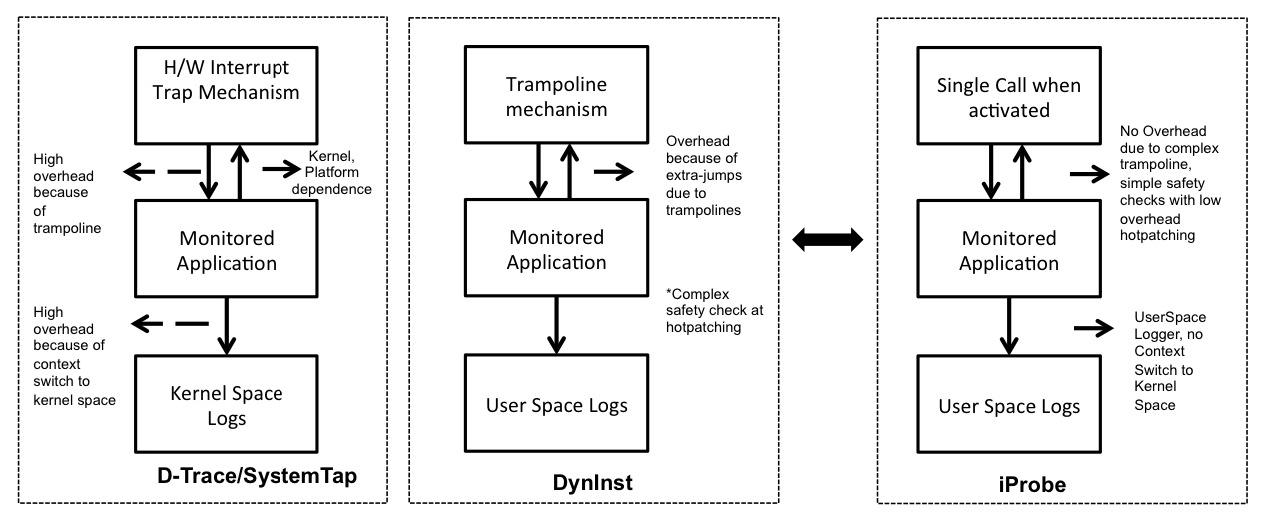
\includegraphics[width=0.9\textwidth]{iprobe/Images/related.eps}
		\caption{Advantages of iProbe over existing monitoring frameworks DTrace/SystemTap and DynInst}
		\label{fig:related}
	\end{center}
\end{figure*}

\subsection{Source Code or Compiler Instrumentation Mechanisms}
Source code instrumentation is one of the most widely available mechanisms for monitoring. 
In essence, users can insert debug statements with runtime flags to dump and inspect program status with varying verbosity levels. 
The log4j~\cite{log4j} and log4c~\cite{log4c} frameworks are commonly used libraries to perform program tracing in many open source projects in the source code level. 
Additionally compilers have several inbuilt profilers which can be used along with tools such as gprof and jprof to gather statistics about program execution.
While source code techniques allow very light weight instrumentation, by design they are static and can only be changed at the start of application execution. 
\iprobe on the other hand offers run-time instrumentation that allows dynamic decisions on tracing with comparable overhead.


\subsection{Run-time Instrumentation Mechanisms}
There are several kernel level tracing tools such as DTrace, LTTng, SystemTap \cite{dtrace,lttng,systemtap} developed by researchers over the years.
\iprobe differs from these approaches mainly in two ways: Firstly, all of these approaches use a technique similar to software interrupt to switch to kernel space and generate a log event by overwriting the target instructions. 
They then execute the instrumentation code, and either generate a trampoline mechanism or re-execute the overwritten target instructions and then jump back to the subsequent instructions. 
As shown in Figure.\ref{fig:related} this introduces context-switches between user-space and the kernel, causing needless overhead. 
iProbe avoids this overhead by having a completely user-space based design.
Secondly, all these approaches require to perform complex checks for correctness which can cause unnecessary overhead at both hotpatching, and when running an instrumented binary. 
%debug information at run-time to find the target function requested by the user. This requirement may not be met in production binaries, and iProbe does not require it in the binaries.

Fay \cite{fay} is a platform-dependent approach which uses the empty spaces at the start of the functions available in Windows binaries for instrumentation. 
To ensure the capture of the entry and exit of functions, Fay calls the target function within its instrumentation thereby introducing an extra stack frame for each target instrumentation. 
This operation is similar to a mini-trampoline and hence incurs an overhead. 
Fay logs function execution in the kernel space and hence also has a context-switch overhead.
\iprobe avoids such overhead by introducing markers at the beginning and end of
each function using a 

Another well known tool is DynInst\cite{dyninst}. This tool provides a rich dynamic instrumentation capability and has pure back box solution towards instrumentation of any application.
However, as shown in Figure.\ref{fig:related} it is also based on traditional trampoline mechanisms, and induces a high overhead because of unnecessary jump instructions.
Additionally it can have higher overhead because of complex security checks. 
Other similar trampoline based tools like \emph{kaho} and \emph{katana}\cite{katana,kaho} have also been proposed, but they focus more towards patching binaries to add \emph{fixes} to correct a bug.

% platform independent 
%compiler technique.

\subsection{Debuggers}
Instrumentation is a commonly used technique in debugging. Many debuggers such as gdb \cite{gdb} and Eclipse have breakpoints and watchpoints which can stop the execution of programs and inspect program conditions. These features are based on various techniques including \texttt{ptrace} and hardware debugging support (single step mode and debug registers). While they provide such powerful instrumentation capabilities, there are in general not adequate for beyond the debugging purposes due to overwhelming overhead.

\subsection{Dynamic Translation Tools}
Software engineering communities have been using dynamic translation tools such as Pin \cite{pin} and Valgrind \cite{valgrind} to inspect program characteristics. 
These tools dynamically translate program code before execution and allow users to insert custom instrumentation code flexibly. They are capable to instrument non-debug binaries and provide versatile tools such as memory checkers and program profilers. However, similar to debuggers, they are generally considered as debugging tools and their overhead is significantly higher than runtime tracers.


